% Copyright 2004 by Till Tantau <tantau@users.sourceforge.net>.

%
% In principle, this file can be redistributed and/or modified under
% the terms of the GNU Public License, version 2.
%
% However, this file is supposed to be a template to be modified
% for your own needs. For this reason, if you use this file as a
% template and not specifically distribute it as part of a another
% package/program, I grant the extra permission to freely copy and
% modify this file as you see fit and even to delete this copyright
% notice. 

\documentclass{beamer}
%% For Citations
\usepackage[natbibapa]{apacite}  % For bibligography
\usepackage{etoolbox}
\usepackage{environ}
\usepackage{subfig}
		
\newtoggle{bibdoi}
\newtoggle{biburl}
\makeatletter
\undef{\APACrefURL}
\undef{\endAPACrefURL}
\undef{\APACrefDOI}
\undef{\endAPACrefDOI}

\togglefalse{bibdoi}\togglefalse{biburl}
\long\def\collect@url#1{\global\def\bib@url{#1}}
\long\def\collect@doi#1{\global\def\bib@doi{#1}}
\newenvironment{APACrefURL}{\global\toggletrue{biburl}\Collect@Body\collect@url}{\unskip\unskip}
\newenvironment{APACrefDOI}{\global\toggletrue{bibdoi}\Collect@Body\collect@doi}{}

\AtBeginEnvironment{thebibliography}{
	\pretocmd{\PrintBackRefs}{%
		\iftoggle{bibdoi}
		{\iftoggle{biburl}{\unskip\unskip doi:\bib@doi}{}}
		{\iftoggle{biburl}{Retrieved from\bib@url}{}}		
		\togglefalse{bibdoi}\togglefalse{biburl}%
	}{}{}
}
% End of DOI or URL but not both code
% Used with the bibspacing.sty to add spacing between bib items
\usepackage{bibspacing}
\setlength{\bibitemsep}{0.75\baselineskip plus .05\baselineskip minus .05\baselineskip}
% End of bibspacing code
%remove the icon
\setbeamertemplate{bibliography item}{}

%remove line breaks
\setbeamertemplate{bibliography entry title}{}
\setbeamertemplate{bibliography entry location}{}
\setbeamertemplate{bibliography entry note}{}
%% End of citations additions

% There are many different themes available for Beamer. A comprehensive
% list with examples is given here:
% http://deic.uab.es/~iblanes/beamer_gallery/index_by_theme.html
% You can uncomment the themes below if you would like to use a different
% one:
%\usetheme{AnnArbor}
%\usetheme{Antibes}
%\usetheme{Bergen}
%\usetheme{Berkeley}
%\usetheme{Berlin}
%\usetheme{Boadilla}
%\usetheme{boxes}
%\usetheme{CambridgeUS}
%\usetheme{Copenhagen}
%\usetheme{Darmstadt}
%\usetheme{default}
%\usetheme{Frankfurt}
%\usetheme{Goettingen}
%\usetheme{Hannover}
%\usetheme{Ilmenau}
%\usetheme{JuanLesPins}
\usetheme{Luebeck}
%\usetheme{Madrid}
%\usetheme{Malmoe}
%\usetheme{Marburg}
%\usetheme{Montpellier}
%\usetheme{PaloAlto}
%\usetheme{Pittsburgh}
%\usetheme{Rochester}
%\usetheme{Singapore}
%\usetheme{Szeged}
%\usetheme{Warsaw}



\setbeamertemplate{footline}
{%
	\leavevmode%
	\hbox{\begin{beamercolorbox}[wd=.2\paperwidth,ht=2.5ex,dp=1.125ex,leftskip=.3cm,rightskip=.3cm plus1fill]{author in head/foot}%
			\usebeamerfont{author in head/foot} \insertframenumber{} / \inserttotalframenumber
		\end{beamercolorbox}%
		\begin{beamercolorbox}[wd=.3\paperwidth,ht=2.5ex,dp=1.125ex,leftskip=.3cm plus1fill,rightskip=.3cm]{author in head/foot}%
			\usebeamerfont{author in head/foot}\insertshortauthor
		\end{beamercolorbox}%
		\begin{beamercolorbox}[wd=.5\paperwidth,ht=2.5ex,dp=1.125ex,leftskip=.3cm,rightskip=.3cm plus1fil]{title in head/foot}%
			\usebeamerfont{title in head/foot}\insertshorttitle
	\end{beamercolorbox}}%
	\vskip0pt%
}


\title{R and Leaflet}
\date{\bfseries Plotting data on a map using R and Leaflet \normalfont \\
	}
\author{Gary R Seamans}
%% Additional Packages
\beamertemplatenavigationsymbolsempty
\setbeamertemplate{headline}{}
\usepackage{xcolor}
\usepackage{mdframed}

\makeatletter
\patchcmd{\@verbatim}
{\verbatim@font}
{\verbatim@font\tiny}
{}{}
\makeatother

% Let's get started
\begin{document}
\begin{frame}
\titlepage
	\begin{figure}
		\centering
		\scalebox{0.035}{
\includegraphics{R_logo.png}}\\
	    \scalebox{0.4}{
\includegraphics{leaflet_logo.png}}
	\end{figure}
\end{frame}

%% New Frame
\begin{frame}{
\begin{minipage}[t]{0.75\textwidth}
	Agenda
\end{minipage}
\hfill
\begin{minipage}[t]{0.25\textwidth}
	\flushright
	\scalebox{0.035}{
\includegraphics{R_logo.png}}
\end{minipage}
}{}
%% ==================== Content ===========================%%
\begin{center}
	\begin{itemize}
		\item Overview of Leaflet
		\item Requirements to use Leaflet
		\item Cleaning the Data
		\item Plotting the Data
		\item Code examples
		\item Questions
	\end{itemize}
\end{center}
\end{frame}

\begin{frame}{
	\begin{minipage}[t]{0.75\textwidth}
		Overview - Leaflet
	\end{minipage}
	\hfill
	\begin{minipage}[t]{0.25\textwidth}
		\flushright
		\scalebox{0.035}{
\includegraphics{R_logo.png}}
	\end{minipage}
}{}
%% ==================== Content ===========================%%
\href{http://leafletjs.com}{\textcolor{blue}{\underline{Leaflet}}} is a lightweight JavaScript library appropriate for general mapping applications including on mobile devices. There is a \href{https://cran.r-project.org/web/packages/leaflet/leaflet.pdf}{\textcolor{blue}{\underline{Leaflet package}}} for R that enables mapping directly from an R application.\\
\vspace{0.5cm}
Today we'll take a quick look at how simple it is to take data from R and place it on a map.

\end{frame}


%% Requirements Frame
\begin{frame}{
	\begin{minipage}[t]{0.75\textwidth}
		Requirements
	\end{minipage}
	\hfill
	\begin{minipage}[t]{0.25\textwidth}
		\flushright
		\scalebox{0.035}{
\includegraphics{R_logo.png}}
	\end{minipage}
}{}
%% ==================== Content ===========================%%
	\begin{itemize}
		\item R, I recommend \href{https://www.rstudio.com/}{\textcolor{blue}{\underline{RStudio}}} 
		\item Packages - We'll cover these in the demo
		\item Data with latitude and longitude information
	\end{itemize}
\end{frame}

%% Cleaning Data
\begin{frame}{
	\begin{minipage}[t]{0.75\textwidth}
		Cleaning Data
	\end{minipage}
	\hfill
	\begin{minipage}[t]{0.25\textwidth}
		\flushright
		\scalebox{0.035}{
\includegraphics{R_logo.png}}
	\end{minipage}
}{}
%% ==================== Content ===========================%%
Cleaning the data involves:
\begin{itemize}
	\item Reading the data into an R dataframe
	\item Taking care of NAs and corrupt data
	\item Making sure the data classes are correct for your purposes
	\item There is a lot more to cleaning data depending on your objective
\end{itemize}

\end{frame}

%% Plotting
\begin{frame}{
	\begin{minipage}[t]{0.75\textwidth}
		Plotting
	\end{minipage}
	\hfill
	\begin{minipage}[t]{0.25\textwidth}
		\flushright
		\scalebox{0.035}{
\includegraphics{R_logo.png}}
	\end{minipage}
}{}
%% ==================== Content ===========================%%
Once the data has been stored in an R dataframe and cleaned you are ready to use Leaflet to plot the data
on a map. This will be covered in more detail during the code review and demo.
\end{frame}

%% Demo and Code
\begin{frame}{
	\begin{minipage}[t]{0.75\textwidth}
		Demo and Code
	\end{minipage}
	\hfill
	\begin{minipage}[t]{0.25\textwidth}
		\flushright
		\scalebox{0.035}{
\includegraphics{R_logo.png}}
	\end{minipage}
}{}
%% ==================== Content ===========================%%
The demo is derived from a project that was part of the Johns Hopkins data science course. The code, and data, has been included in this repository or you can clone it directly from my public GitHub repository at \href{https://github.com/gseamans/starbucksUsa}{\textcolor{blue}{\underline{Seamans - StarbucksUSA}}}. There are a number of other public projects from the data science course in my GitHub repository. Feel free to clone any of them.

\end{frame}

%% Links
\begin{frame}{
	\begin{minipage}[t]{0.75\textwidth}
		Links
	\end{minipage}
	\hfill
	\begin{minipage}[t]{0.25\textwidth}
		\flushright
		\scalebox{0.035}{
\includegraphics{R_logo.png}}
	\end{minipage}
}{}
%% ==================== Content ===========================%%
\begin{itemize}
	\item \href{https://github.com/gseamans/starbucksUsa}{\textcolor{blue}{\underline{StarbucksUSA GitHub}}}
	\item \href{https://gseamans.shinyapps.io/starbucksusa/}{\textcolor{blue}{\underline{StarbucksUSA Shiny App}}}
	\item \href{https://github.com/gseamans/Starbucks-In-Arizona}{\textcolor{blue}{\underline{Starbucks-In-Arizona GitHub}}}
	\item \href{https://gseamans.github.io/Starbucks-In-Arizona/}{\textcolor{blue}{\underline{Starbucks-In-Arizona WebPage}}}
	\item \href{https://www.openstreetmap.org/\#map=4/38.01/-95.84}{\textcolor{blue}{\underline{OpenStreetMap}}}
\end{itemize}

\end{frame}

\usebackgroundtemplate{
	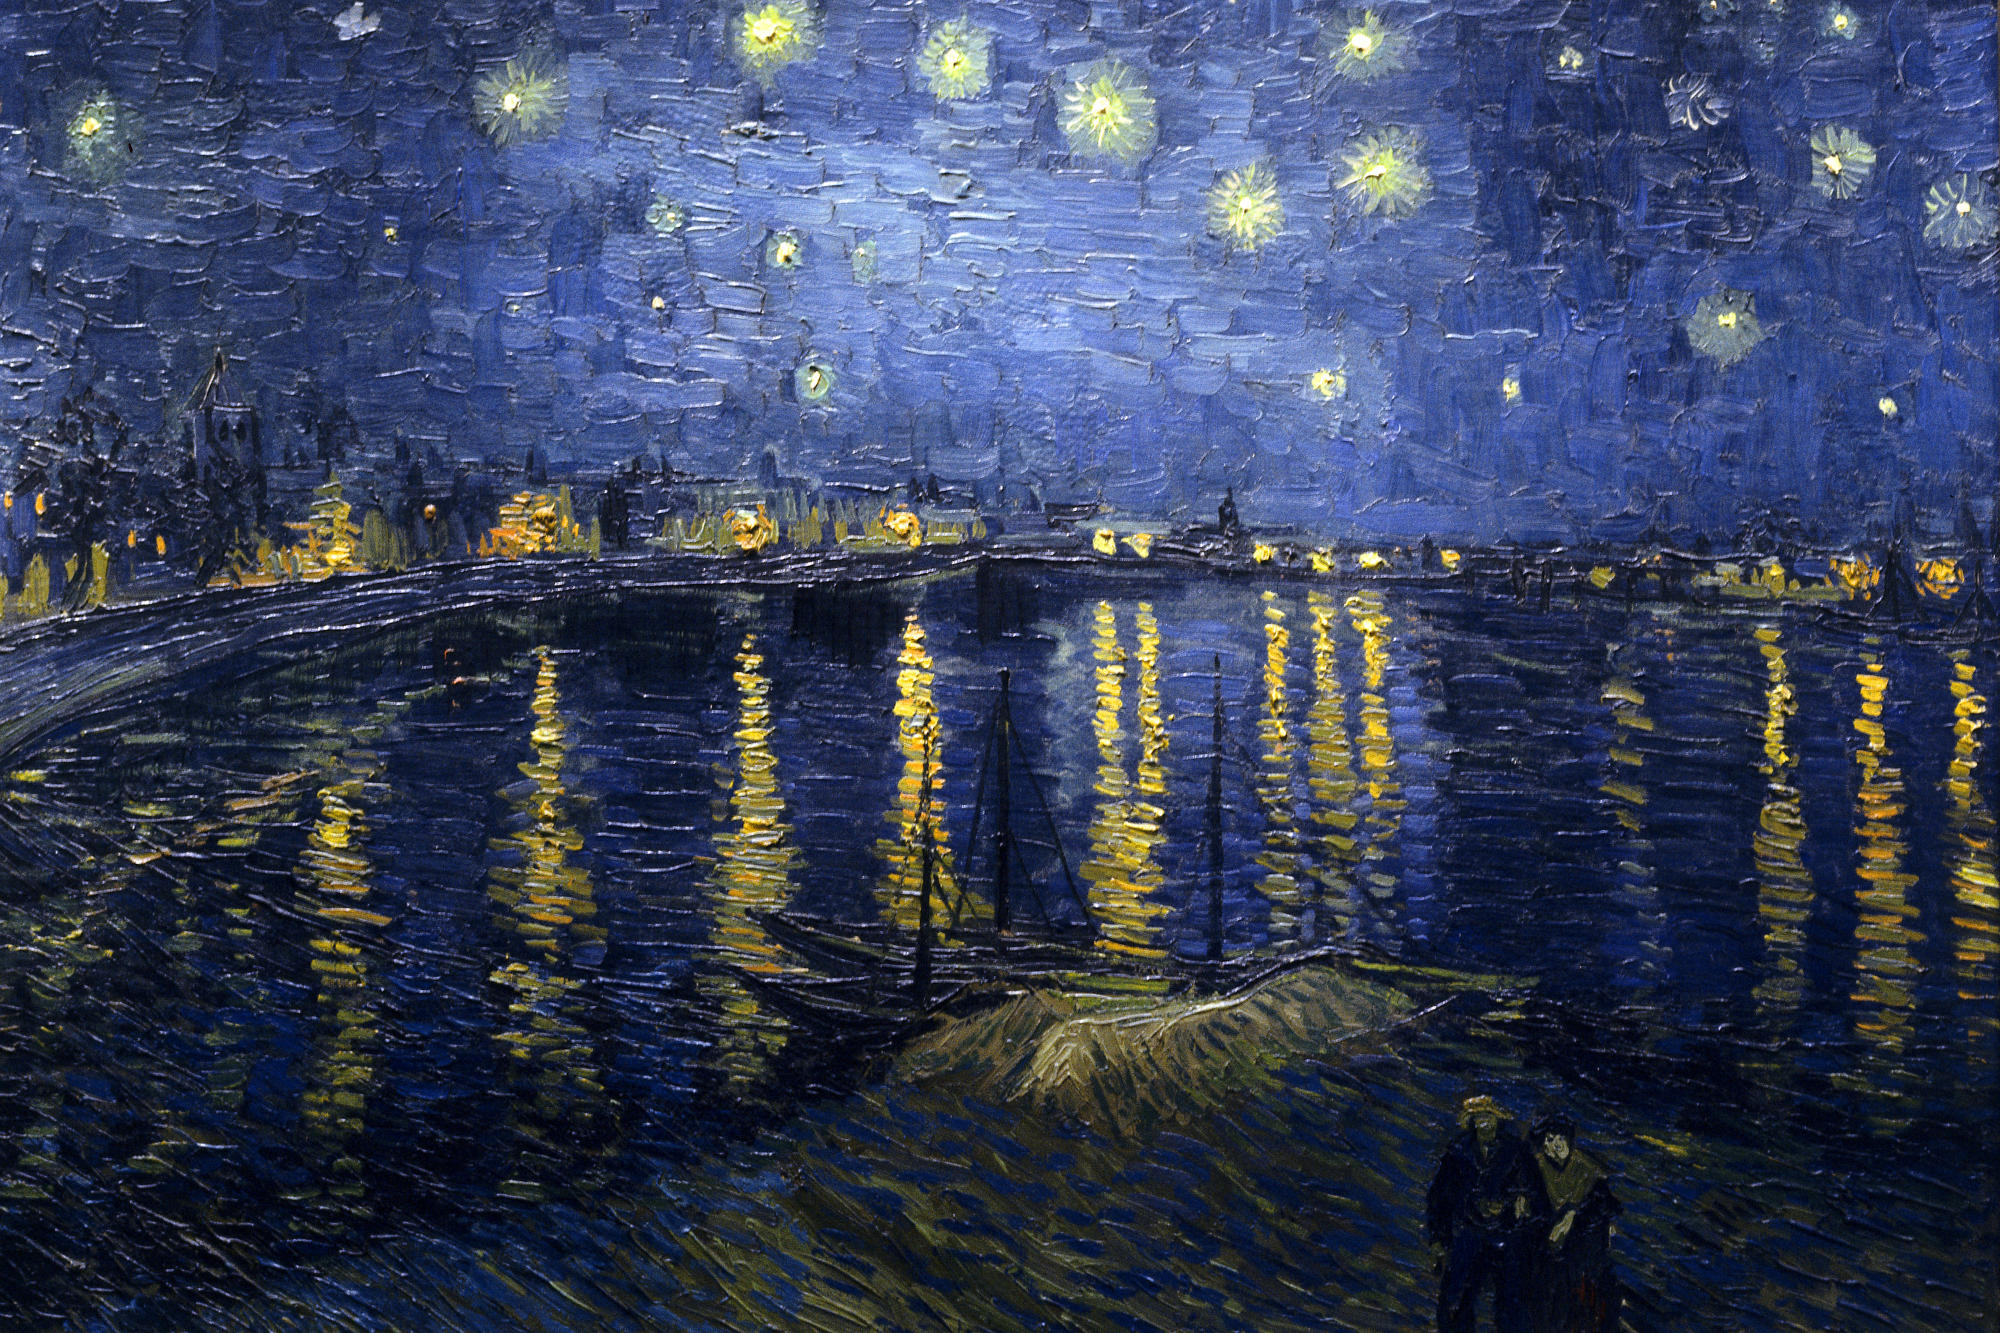
\includegraphics[width=\paperwidth]{starryrhone_vangogh_big.jpg}}
%% Questions
\begin{frame}{
	\begin{minipage}[t]{0.75\textwidth}
		Questions
	\end{minipage}
	\hfill
	\begin{minipage}[t]{0.25\textwidth}
		\flushright
		\scalebox{0.035}{
\includegraphics{R_logo.png}}
	\end{minipage}
}{}
%% ==================== Content ===========================%%

\end{frame}

\usebackgroundtemplate{
	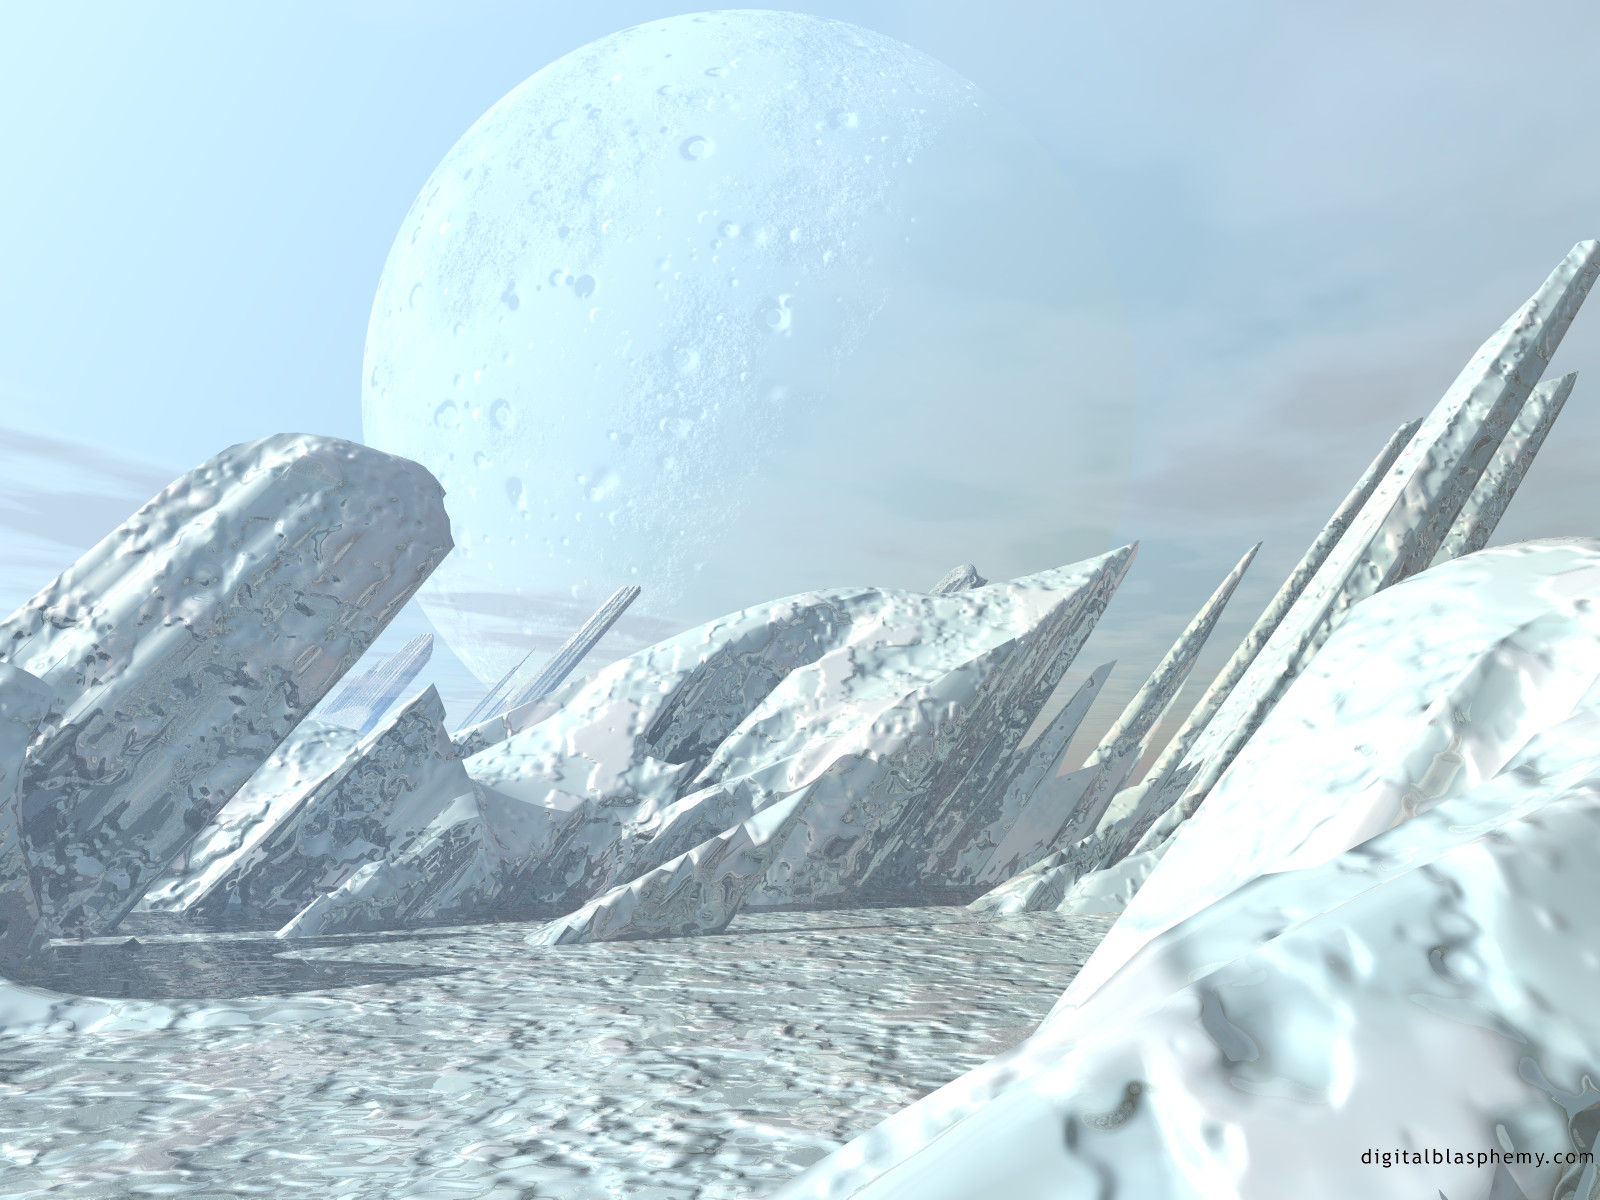
\includegraphics[width=\paperwidth]{borealis1600.jpg}}
%% Future Brownbags
\begin{frame}{
	\begin{minipage}[t]{0.75\textwidth}
		R Brown Bags
	\end{minipage}
	\hfill
	\begin{minipage}[t]{0.25\textwidth}
		\flushright
		\scalebox{0.035}{
\includegraphics{R_logo.png}}
	\end{minipage}
}{}
%% ==================== Content ===========================%%
	\begin{itemize}
		\item Documentation with R - Knitr (Scheduled for 31 January 1130 - 1215)
		\item Installing RStudio
		\item Data loading from (flat files in various formats, databases)
		\item Integrating R with Big Data sources.
		\item Data cleaning
		\item Statistical Inference (Would need to be split up.)
		\item Machine learning (would need to be split up in to several, e.g. Intro including partitioning/cleaning datasets, Random Forests, Naïve Bayes, Boosting \& Bagging, etc) 
		\item Exploratory data analysis techniques
		\item Regression modelling
		\item Creating custom R packages
		\item Misc topics including RStudio (feeding and maintenance), Shiny, Plotly, etc.
	\end{itemize}
\end{frame}

%% Software Security
\begin{frame}{
	\begin{minipage}[t]{0.75\textwidth}
		Software Security  Brown Bags
	\end{minipage}
	\hfill
	\begin{minipage}[t]{0.25\textwidth}
		\flushright
		\scalebox{0.035}{
\includegraphics{R_logo.png}}
	\end{minipage}
}{}
%% ==================== Content ===========================%%
	\begin{itemize}
		\item Using Kali
		\item Overview of software security best practices (development) 
		\item Penetration testing
		\item Overview of tools for developing/analyzing secure software
	\end{itemize}

\end{frame}

%% General Topics
\begin{frame}{
	\begin{minipage}[t]{0.75\textwidth}
		General Topics Brown Bags
	\end{minipage}
	\hfill
	\begin{minipage}[t]{0.25\textwidth}
		\flushright
		\scalebox{0.035}{
\includegraphics{R_logo.png}}
	\end{minipage}
}{}
%% ==================== Content ===========================%%
\begin{itemize}
	\item Graph databases, both first order semantic stores and property graphs (overview and comparison)
	\item Ontology creation
	\item Designing a property graph
	\item Tool overview
	\item BDP overview
	\item Graph database for analysing network assets
\end{itemize}

\end{frame}

\end{document}